\section{Les processus}

	\subsection{Définitions}
		Un processus est programme en cours d'exécution auquel est associé un environnement processeur et un environnement mémoire. En effet, au cours de son exécution, les instructions d'un programme modifient les valeurs des registres (compteur ordinal, registre d'état...) ainsi que le contenu de la pile.\\
		Un programme est une suite d'instructions (notion statique), tandis qu'un processus, c'est l'image du contenu des registres et de la mémoire centrale (notion dynamique).
	
		\paragraph{} Chaque processus possède un \textit{\textbf{espace d'adressage}}, c'est-à-dire un ensemble d'adresses mémoires dans lesquelles il peut lire et écrire. Cet espace est divisé en trois parties :
		\begin{itemize}
			\item le segment de texte (le code du programme)
			\item le segment de données (les variables)
			\item la pile
		\end{itemize}
		
		\begin{center}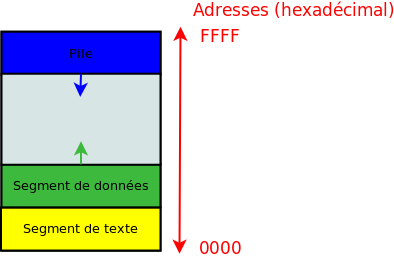
\includegraphics[scale=0.8]{../img/adr.png}\end{center}
		L'espace vide au milieu permet à la pile de s'étendre dessus de manière automatique et au segment de données de faire une extension lors d'une allocation dynamique.
			
		\paragraph{}
		Lorsqu'un processus est lancé, le système doit gérer la mémoire et l'allocation du processeur lui étant accordée. Il fait appel à l'\textit{\textbf{ordonnanceur}}.\\
		Un système d'exploitation est multitâche \textbf{\textit{préemptif}} lorsqu'il peut arrêter à tout moment n'importe quelle application pour passer à la suivante (Windows XP, Windows 7 et GNU/Linux). Il garde donc le contrôle et se réserve le droit de fermer l'application.\\
		Un système d'exploitation est multitâche \textbf{\textit{coopératif}} quand il permet à plusieurs applications de fonctionner et d'occuper la mémoire, et leur laissant gérer cette occupation (Windows 95, 98 et Millénium).\\
		Les systèmes basés sur UNIX sont tous des systèmes préemptifs.
		
	\subsection{Gestion des processus sous UNIX}
		Dans les systèmes basés sur UNIX particulièrement, les processus jouent un rôle très important. Le concept de processus a été mis au point dès les débuts de ce système : il a ainsi participé à sa gloire et à sa célébrité. Une des particularités de la gestion des processus sous UNIX consiste à séparer la création d'un processus et l'exécution d'une image binaire. Bien que la plupart du temps ces deux tâches sont exécutées ensemble, cette division a permis de nouvelles libertés quant à la gestion des tâches. Par exemple, cela permet d'avoir plusieurs processus pour un même programme.\\
		
		Autrement dit, sous les autres systèmes d'exploitation (mis à part quelques exceptions), un processus est l'équivalent d'un nouveau programme, alors que sous UNIX ce n'est pas forcément le cas.\\
		Ce principe, peu utilisé dans les autres systèmes, a survécu de nos jours. Alors que la plupart des systèmes d'exploitation offrent un seul appel-système pour exécuter un nouveau programme, UNIX en possède deux : \lstinline!fork! et \lstinline!exec!.\\
		
		La commande \lstinline!ps! permet d'afficher ses propres processus en cours d'exécution. Pour afficher tous les processus en cours d'exécution, on utilise l'option \lstinline!aux! (a : processus de tous les utilisateurs, u : affichage détaillé, x : démons).
		
		\subsubsection*{PID :}
			Chaque processus peut être identifié par son numéro de processus, ou PID (\textbf{\textit{Process IDentifier}}). Un numéro de PID est unique dans le système : il est impossible que deux processus aient un même PID au même moment.\\
			Lorsque l'on crée un processus, on utilise une fonction qui permet de dupliquer le processus appelant. On distingue alors les deux processus par leur PID. Le processus appelant est alors nommé \textbf{processus père} et le nouveau processus \textbf{processus fils}. Quant on s'occupe du processus fils, le PID du processus père est noté \textbf{PPID} (\textbf{\textit{Parent PID}}).\\
			
			Par défaut, le noyau attribue un PID avec une valeur inférieure à 32768. Le 32768ème processus créé reçoit la plus petite valeur de PID libéré par un processus mort entre-temps. Cette valeur maximale peut être changée par l'administrateur en modifiant la valeur du fichier \lstinline!/proc/sys/kernel/pid_max!.\\
			De plus, les PID sont attribués de façon linéaire. Par exemple, si 17 est le PID le plus élevé affecté, un processus créé à cet instant aura comme PID 18. Le noyau réutilise les PID de processus n'existant plus uniquement quand la valeur de \lstinline!pid_max! est atteinte.
			
		\subsubsection*{Organisation des processus :}
			Les processus sont organisés en \textbf{\textit{hiérarchie}}. Chaque processus doit être lancé par un autre (processus père et processus fils). La racine de cette hiérarchie est le programme initial.\\ 
			En effet, le processus inactif du système (\textbf{\textit{System idle process}} processus que le noyau exécute tant qu'il n'y a pas d'autres processus en cours d'exécution) a le PID 0. C'est celui-ci qui lance le premier processus que le noyau exécute, le programme initial. Généralement, sous les systèmes basés sous UNIX, le programme initial se nomme \lstinline!init!, et il a le PID 1.
			
			Si l'utilisateur indique au noyau le programme initial à exécuter, celui-ci tente alors de le faire avec quatre exécutables, dans l'ordre suivant : \lstinline!/sbin/init!, \lstinline!/etc/init! puis \lstinline!/bin/init!. Le premier de ces processus qui existe est exécuté en tant que programme initial. Si les quatre programmes n'ont pas pu être exécutés, le système s'arrête. Après son chargement, le programme initial gère le reste du démarrage : initialisation du système, lancement d'un programme de connexion... Il se charge également de lancer les démons. Un démon (\textbf{\textit{daemon}}) est un processus qui est constamment en activité et fournit des services au système.

		\subsubsection*{États d'un processus :}
			Un processus peut avoir plusieurs états :
			\begin{itemize}
				\item exécution (R pour running) : le processus est en cours d'exécution
				\item sommeil (S pour sleeping) : dans un multitâche coopératif, quand il rend la main, ou dans un multitâche préemptif, quand il est interrompu au bout d'un quantum de temps
				\item arrêt (T pour stopped) : le processus a été temporairement arrêté par un signal, il ne s'exécute plus et ne réagira qu'à un signal de redémarrage
				\item zombie (Z pour … zombie) : le processus fils (zombie) s'est terminé avant le père
			\end{itemize}
			Sous UNIX, un processus peut évoluer dans deux modes différents : le mode noyau et le mode utilisateur. Généralement, un processus utilisateur entre dans le mode noyau quand il effectue un appel-système.
			
			\begin{center}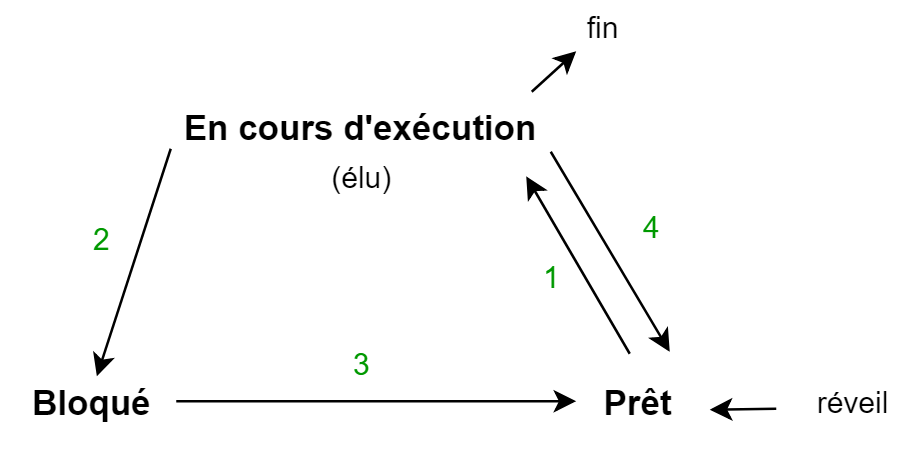
\includegraphics[scale=0.4]{../img/process.png}\end{center}
			
			\begin{itemize}
				\item 1 : élection, l'ordonnanceur choisit ce processus
				\item 2 : blocage, processus bloqué en attente d'une donnée
				\item 3 : déblocage, donnée devient disponible
				\item 4 : l'ordonnanceur choisit un autre processus
			\end{itemize}
			
		\subsubsection*{Implémentation d'un processus :}
			Pour implémenter les processus, le système d'exploitation utilise un tableau de structure, appelé \textbf{table des processus}. Cette table comprend une entrée par processus, allouée dynamiquement, correspondant au processus associé à ce programme : c'est le bloc de contrôle du processus (\textbf{\textit{Process Control Block}}, PCB). Ce bloc contient, entres autres, les informations suivantes :
			\begin{itemize}
				\item le PID, le PPID, l'UID (identifiant de l'utilisateur) et le GID (identifiant du groupe, chaque utilisateur du système appartient à un ou plusieurs groupes) du processus
				\item l'état du processus
				\item les fichiers ouverts par le processus
				\item le répertoire courant du processus
				\item le terminal attaché au processus
				\item les signaux reçus par le processus
				\item le contexte processeur et mémoire du processus (l'état des registres et des données mémoires du processus)
			\end{itemize}
			Grâce à ces informations stockées dans la table des processus, un processus bloqué pourra redémarrer ultérieurement avec les mêmes caractéristiques.
			
			
	\subsection{Manipulation des processus en C}
		\subsubsection{Création d'un processus :}
			Pour créer un nouveau processus à partir d'un programme, on utilise la fonction système \lstinline!fork!. 
			\begin{lstlisting}
				#include <unistd.h>
				#include <sys/types.h>

				pid_t fork(void);
			\end{lstlisting}
			Le processus d'origine est le processus père et le nouveau processus créé est le processus fils, qui possède un nouveau PID. Les processus deux ont le même code source, mais la valeur retournée par \lstinline!fork! nous permet de savoir si l'on est dans le processus père ou dans le processus fils. Ceci permet de faire deux choses différentes dans le processus père et le processus fils.\\
			Lors de l'exécution de l'appel-système \lstinline!fork!, le noyau effectue les opérations suivantes :
			\begin{itemize}
				\item alloue un bloc de contrôle dans la table des processus
				\item copie les informations contenues dans le bloc de contrôle du père dans celui du fils sauf les identificateurs (PID, PPID...)
				\item alloue un PID au processus fils
				\item associe au processus fils un segment de texte dans son espace d'adressage. Le segment de données et la pile ne lui seront attribués uniquement lorsque celui-ci tentera de les modifier. Cette technique, nommée copy on write, permet de réduire le temps de création du processus
				\item l'état du processus est mis à l'état exécution
			\end{itemize}
			
			\noindent La fonction \lstinline!fork! retourne :
			\begin{itemize}
				\item -1 en cas d'erreur
				\item 0 si on est dans le processus fils
				\item le PID du fils si on est dans le processus père. Cela permet ainsi au père de connaître le PID de son fils
			\end{itemize}
			
			\noindent \textbf{Autres fonctions :}
			\begin{lstlisting}
				#include <unistd.h>
				#include <sys/types.h>

				pid_t getpid(void);
				// retourne le PID du processus appelant
				
				pid_t getppid(void);
				// retourne le PPID du processus appelant
			\end{lstlisting}
			
		\subsubsection{Terminaison d'un processus :}
			Un programme peut se terminer normalement de deux façons différentes. La plus simple consiste à laisser le processus finir le \lstinline!main! avec l'instruction \lstinline!return! suivie du code de retour du programme. Une autre façon est de terminer le programme grâce à la fonction \lstinline!exit()! depuis n'importe quelle fonction.
			\begin{lstlisting}
				#include <stdlib.h>

				void exit(status);
			\end{lstlisting}
			Un programme peut aussi se terminer de façon anormale, en cas d'erreur par exemple. Pour cela, on peut utiliser les fonctions \lstinline!abort(void)! ou \lstinline!assert(int condition)! par exemple. 
			
			
		\subsubsection{Synchronisation entre processus :}
			Un processus \textbf{zombie} est un processus qui s'est achevé, mais qui dispose toujours d'un identifiant de processus (PID) et reste donc encore visible dans la table des processus. Lorsque le processus fils se termine avant le processus père (c'est à dire que le père n'a pas encore lu le code de retour du fils), le processus fils devient un zombie.\\
			
			Pour permettre à un processus fils zombie de disparaître complètement, on utilise la fonction \lstinline!wait()!.
			\begin{lstlisting}
				#include <sys/types.h>
				#include <sys/wait.h>

				pid_t wait(int* status);
			\end{lstlisting}
			Lorsque l'on appelle cette fonction, celle-ci bloque le processus à partir duquel elle a été appelée (père) jusqu'à ce qu'un de ses fils se termine. Elle renvoie alors le PID de ce dernier. En cas d'erreur, la fonction renvoie la valeur -1.\\
			Le paramètre \lstinline!status! correspond au code de retour du processus (ce code de retour est généralement indiqué avec la fonction exit).\\
			Il faut veiller à mettre autant de \lstinline!wait! dans le père qu'il a de processus fils.\\
			
			Sans la fonction \lstinline!wait!, le processus père s'arrête sans avoir lu le code de retour de son fils qui va devenir (ou rester s'il est déjà terminé) zombie. La seule manière d'éliminer ce processus zombies est de causer la mort du processus père (si ce n'est pas déjà fait). Les processus fils sont alors automatiquement rattachés au processus au PID 1, généralement \lstinline!init!, qui se charge à la place du père original d'appeler \lstinline!wait! sur ces derniers. Si ce n'est pas le cas, cela signifie que \lstinline!init! est défaillant (ou que le processus 1 n'est pas \lstinline!init!, mais un autre programme n'ayant pas été prévu pour ça) et le seul moyen de se débarrasser des zombies, dans ce cas, est le redémarrage du système.
			
			\paragraph{La fonction \lstinline!waitpid! :} permet de suspendre l'exécution d'un processus père jusqu'à ce qu'un de ses fils, dont on doit passer le PID en paramètre, se termine.
			\begin{lstlisting}
				#include <sys/wait.h>

				pid_t waitpid(pid_t pid, int* status, int options);
				\\waitpid(-1, status, 0) correspond à wait
			\end{lstlisting}
			\begin{itemize}
				\item si pid > 0, le processus père est suspendu jusqu'à la fin d'un processus fils dont le PID est égal à la valeur pid
				\item si pid = 0, le processus père est suspendu jusqu'à la fin de n'importe lequel de ses fils appartenant à son groupe
				\item si pid = -1, le processus père est suspendu jusqu'à la fin de n'importe lequel de ses fils
				\item si pid < -1, le processus père est suspendu jusqu'à la mort de n'importe lequel de ses fils dont le GID est égal
				\item \lstinline!status! a le même rôle qu'avec \lstinline!wait!
				\item \lstinline!options! permet de préciser le comportement de \lstinline!waitpid! : WNOHANG (ne pas bloquer si aucun fils ne s'est terminé), WUNTRACED (recevoir l'information concernant également les fils bloqués si on ne l'a pas encore reçue) ou 0.
			\end{itemize}
			
			
		\subsubsection*{Exemple :}
			\begin{center}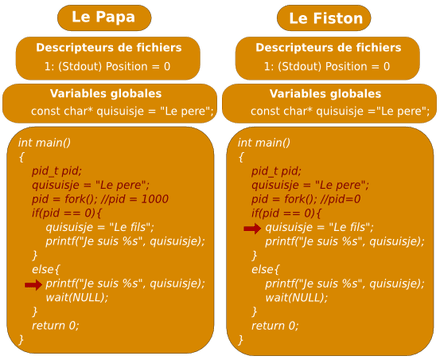
\includegraphics[scale=0.8]{../img/fork1.png}\end{center}
			\begin{center}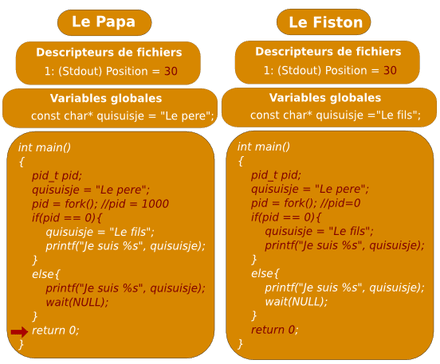
\includegraphics[scale=0.8]{../img/fork2.png}\end{center}
			La variable \lstinline!quiSuisJe! va être modifiée pour le processus fils seulement. La position de \lstinline!stdout! va avancer de 15 caractères pour le \lstinline!printf! du père et 15 autres caractères pour le \lstinline!printf! du fils pour valoir 30 au final pour les deux processus.\\
			Les variables du processus père et celles du fils sont totalement distinctes. Par contre, leur descripteurs de fichiers sont les mêmes. Donc, si l'un des deux processus modifie son pointeur de position dans un fichier, ça se répercutera également chez l'autre. Cela ne vaut que pour les descripteurs de fichiers hérités durant le \lstinline!fork!, c'est-à-dire, si le père ou le fils ouvre d'autres fichiers après le \lstinline!fork!, ces descripteurs ne seront pas partagés entre eux deux. De même, si le fils ferme un descripteur de fichier hérité du père, le descripteur de fichier du père ne sera par contre pas fermé (même chose dans le sens inverse).\\
			~\\
			\noindent On ne peut pas savoir quel processus va s'exécuter en premier. Pour la fonction \lstinline!wait!, il est préférable l'utiliser ainsi :
			\begin{lstlisting}
				if ( wait(NULL) == -1 )
					perror("wait");
			\end{lstlisting}
				
		
		
		